\documentclass[11pt,letterpaper]{article}
\usepackage[utf8]{inputenc}
\usepackage[spanish]{babel}
\usepackage{fancyvrb}
\usepackage{fancyhdr}
\usepackage{graphicx}
\usepackage{amsmath}

\title{}
\author{}

\parskip 1mm %Espacio entre parrafos
\setlength{\topmargin}{0pt}
\oddsidemargin	0.5cm  % Ancho Letter 21,59cm
\evensidemargin 0.5cm  % Alto  Letter 27,81cm
\textwidth	15.5cm
\textheight	21.0cm
\headsep	4 mm
\parindent	0.5cm

\pagestyle{fancyplain}

\lhead{Computación Científica 1} %Parte superior izquierda
\rhead{\bf \it 2009} %Parte superior derecha
\lfoot{} %Parte inferior izquierda. \thepage indica el numero de pagina
\cfoot{} %Parte inferior central
\rfoot{\bf \thepage} %Parte inferior derecha
\renewcommand{\footrulewidth}{0.4pt} %Linea de separacion inferior

\makeatother

\begin{document}

%  identificación de los proponentes, nombre de la pre-Empresa y del Producto.

\begin{titlepage}
    \begin{center}
	\begin{tabular}{ccc}
	    
\includegraphics[width=3cm]{img/utfsm}
	    & 
	    \hspace{-0.2cm}
	    \begin{tabular}{c}
		Universidad Técnica Federico Santa María \\ \hline
		\vspace{0.2cm}
		Departamento de Informática\\
		\vspace{1.2cm}
	    \end{tabular}
	    \hspace{0.2cm}
	    &
            
\includegraphics[width=2cm]{img/di}
	\end{tabular}

	\vspace{1cm}
	%Titulo del Documento
	\begin{tabular}{c}
		\Huge{\sc{Computación Científica I}}\\\\\\\\\\
		\huge{\sc{Informe Laboratorio II}}
	\end{tabular}
		\vspace{5cm}
	\\
	\begin{tabular}{c}
		\Large{\sc{Integrantes}}
		\vspace{1cm}
	\end{tabular}
	\\
	\begin{tabular}{cr}
         	\large{Gabriel Zamora Nelson}      & \footnotesize \emph{Rol: 2673070-8}\\
         	\large{Cristián Maurerira Fredes}  & \footnotesize \emph{Rol: 2673030-9}\\
         	\large{Rodrigo Fernández Gaete} 	& \footnotesize \emph{Rol: 2673002-3}\\
	\end{tabular}
	\\
	\vspace{\fill}
	%Fecha
		\normalsize{\sc{Valparaíso, Julio 2009}}\\
    \end{center}
\end{titlepage}


\section{Vectores}
\begin{enumerate}
	\item Genere dos vectores aleatorios $R$, $S$ de tamaño $1x11$, tal que cada uno de sus elementos
		sean números primos pertenecientes al intervalo $[1,\ldots,211]$.

	\textbf{R:}\\

R = [37 13 163 131 137 199 139 173  79  47 139] \\
S = [139 173  43 103 173  47  89 109  37 181  83] \\
 
	\item Calcule el valor de $RxS$, $R.S$, $R*S'$, ¿Cual es la diferencia entre cada una de estas
operaciones?, ¿existe alguna información útil que podamos saber de estas?.

	\textbf{R:}\\

	El producto cruz normalmente está definido sólo para $R^3$,
	de todas formas es posible calcularlo para un espacio de $n$ dimensiones,
	pero es necesario contar con al menos $n-1$ vectores,
	finalmente no se puede realizar, ya que falta información\\

	$R$.$S$ = 115143 \\
	$R$*$S$' = 115143 \\

	Dado que los componentes de los vectores, el operador conjugación no realiza grandes cambios en los componentes en si de $S$, 
	por lo que se obtiene una operación equivalente.

	\item Calcule un Vector normal para el vector $R$ y para el vector $S$.

	\textbf{R:}\\

	Para calcular un vector normal N a $R$ y $S$, debe cumplirse que: \\

	$R$.$N_1$ = 0 \\
	$S$.$N_2$ = 0 \\

	Debido a que poseemos 11 incógnitas y 1 ecuación en cada caso, asumimos cualquier valor para los primeros 
	10 componentes del vector N, para luego despejar el componente 11: \\

	$N_1$ = [1.0 1.0 1.0 1.0 1.0 1.0 1.0 1.0 1.0 1.0 -8.0432] \\
	$N_2$ = [1.0  1.0  1.0  1.0  1.0  1.0  1.0  1.0  1.0  1.0 -13.1807] \\
	\newpage
	\item Calcule el ángulo entre los vectores generados.

	\textbf{R:}\\

	$R.S = |R||S| Cos(\phi)$
	$\Leftrightarrow \phi = Cos^{-1}\frac{R.S}{|R||S|} = 46.463^{\circ}$\\

	\item Genere dos vectores con las primeras 3 columnas de $R$ y $S$, grafique los dos nuevos vectores,
		identifique de forma clara cada uno de los vectores.

	\textbf{R:}\\

	r = [37  13 163] \\
	s = [139 173  43] \\

	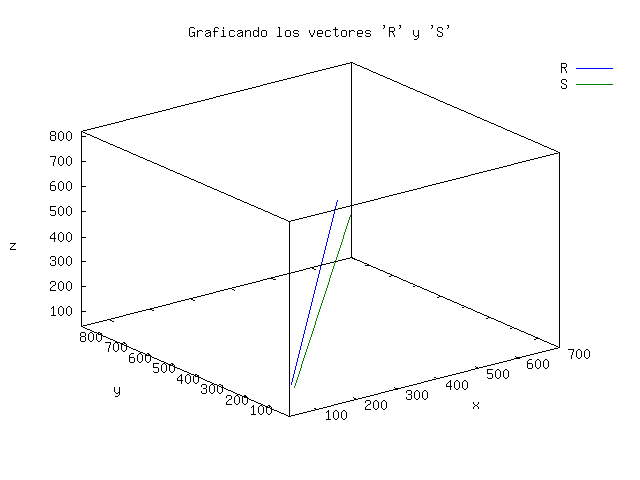
\includegraphics[scale=0.6]{imagenes/vectores.png}

\end{enumerate}


\newpage

\section{Matrices}
\begin{enumerate}
	\item Genere una matriz de $7x7$ que contenga sólo números
	primos ordenados de menor a mayor.\\
	\textbf{R:}\\
\begin{center}
$
\begin{bmatrix}
     2 &    3 &    5 &    7 &   11 &   13 &   17\\ 
    19 &   23 &   29 &   31 &   37 &   41 &   43\\
    47 &   53 &   59 &   61 &   67 &   71 &   73\\
    79 &   83 &   89 &   97 &  101 &  103 &  107\\
   109 &  113 &  127 &  131 &  137 &  139 &  149\\
   151 &  157 &  163 &  167 &  173 &  179 &  181\\
   191 &  193 &  197 &  199 &  211 &  223 &  227
\end{bmatrix}
$
\end{center}
	\item Encuentre los valores propios de la matriz generada,
	 usando la función provista por el software.\\
	\textbf{R:}\\
$
\lambda_1 = 741.95179 + 0.00000i\\ 
\lambda_2 = -26.71104 + 0.00000i\\
\lambda_3 =   5.00551 + 1.16550i\\
\lambda_4 =   5.00551 - 1.16550i\\
\lambda_5 =   0.78161 + 0.00000i\\
\lambda_6 =  -1.01669 + 0.04980i\\
\lambda_7 =  -1.01669 - 0.04980i\\
$
	\item Implemente un algoritmo que encuentre los valores propios
	de la matriz generada.\\
	\textbf{R:}\\
	El algoritmo que utilizamos,
	está basado en obtener el polinomio característico,
	y luego obtener las raíces de dicha ecuación.\\
	\begin{verbatim}
	octave:1> roots(poly(m))
	\end{verbatim}
	Donde $m$, es la matriz con la cual estamos trabajando.\\
	$poly(m)$ obtiene un vector con los coeficientes del polinomio característico y
	$roots(m)$ obtiene las raíces de un polinomio determinado.
	
	\item Compare los resultados obtenidos de su función contra la
	función provista por el software.\\
	\textbf{R:}\\
	Los resultados para nuestra matriz de $7x7$
	en ambos casos fueron iguales,
	ésto es debido a que de las dos formas se utilizan funciones provistas por octave.\\


	\item Poniendo a prueba a los algoritmos: compare los tiempos de respuestas de su algoritmo,
		realice varios experimentos aumentando el tamaño de la matriz progresivamente hasta un
		tamaño razonable.
	\begin{enumerate}
 		\item ¿Cómo se comporta su algoritmo a medida que el tamaño de la matriz aumenta?\\
		\textbf{R:}\\
		Nuestro algoritmo soporto sólo hasta una matriz de $507x507$,
		ésto se debe a las limitaciones que tiene el comando $roots()$,
		lo cuál nos llamo mucho la atención ya que como los provee el mismo programa,
		uno piensa que son 100\% eficientes, pero si nos damos cuenta
		resolver una ecuación de grado $507$ es todo un reto.
		\begin{verbatim}
		roots(poly(rand(507)))
		\end{verbatim}
		Para valores aceptados muy grandes,
		se demora aproximadamente $5$ segundos en poder entregar la solución.

		\item ¿Sucede lo mismo con el algoritmo que utiliza la función del software, por qué?\\
		\textbf{R:}\\
		El algoritmo del software $eig()$ se demora mucho menos en poder obtener los
		valores propios, alrededor de $2$ segundos.
		Lo cual claramente es un signo de que cuando un algoritmo está enfocado a una tarea
		en especial, es mucho mas eficiente comparado con la forma $inadecuada$ que pudimos
		plantear para obtener el resultado.

		\item ¿Qué es un tamaño razonable?
		\textbf{R:}\\
		Un tamaño razonable con respecto a éste problema,
		es un tamaño que transforma la simple tarea de realizar
		\emph{a mano} algún algoritmo para obtener valores propios,
		en un ejercicio \emph{inhumano} y casi imposible de realizar.

		Nadie en su sano juicio,
		sería capaz de realizar el algoritmo con el polinomio característico
		para obtener valores propios de una matriz de $500x500$

	\end{enumerate}
	\item Encuentre los vectores linealmente independientes de la matriz generada en $(2.1)$.\\
	\textbf{R:}\\
	Como la matriz que formamos está compuesta sólo con números primos,
	no existe la posibilidad de que existan múltiplos de algunos vectores,
	y que lleguemos a la conclusión de que dos vectores son \emph{linealmente dependiente}.

	Por lo tanto todos los vectores de la matriz son \emph{linealmente independientes}.

	Una manera de comprobarlo,
	es operando la matriz hasta poder llegar a su forma irreductible.
	Ésto es posible mediante la siguiente sentencia de \emph{octave}\\
	\begin{verbatim}
	octave:1> ((rref(m')))'
	\end{verbatim}
	Lo que quiere decir, que trasponemos la matriz, realizamos operaciones filas,
	finalmente la trasponemos nuevamente, para dejarla en su estado inicial, y el
	resultado que nos estrega es la matriz de identidad de dimensiones $7x7$,
	lo que quiere decir, que llegamos a las bases canónicas, comprobando así
	que \emph{todos} sus vectores son \emph{linealmente independientes}
	
	
	

	\item ¿Puede dar un ejemplo de una matriz cuyos vectores sean ortogonales pero que no sean
		linealmente independientes? Demuestre.\\
		\textbf{R:}\\
		Supongamos que existe un conjunto ortogonal $ x_1,x_2,\cdots,x_k$ y construyamos una combinación
		lineal nula de ellos:

		$\displaystyle \alpha_1x_1+\alpha_2x_2+\cdots+\alpha_nx_n=0 $

		Si seleccionamos un vector cualquiera $ x_j$ y efectuamos el producto interno a cada lado
		de la ecuación tenemos

		$\displaystyle \alpha_1P(x_1,x_j)+\alpha_2P(x_2,x_j)+\cdots+\alpha_nP(x_n,x_j)=0 $

		Como se trata de un sistema ortogonal, el único $ P(x_i,x_j)\neq 0$ es $ P(x_j,x_j)=P_i$, y
		por lo tanto

		$\displaystyle \alpha_jP(x_j,x_j)=\alpha_jP_i=0 $

		Y por tanto

		$\displaystyle \alpha_j=0 $

		Por lo que podemos concluir que la única combinación lineal nula de los vectores es la
		que tiene coeficientes nulos, es decir, los vectores son linealmente independientes.

\end{enumerate}



\newpage

\section{Transformaciones Lineales}
	Sea la transformación $R$:
	\[
	R(\theta) = \begin{bmatrix} \cos \theta & -\sin \theta \\[3pt] \sin \theta & \cos \theta \\ \end{bmatrix}
	\]

\begin{enumerate}
	\item Genere y grafique un Vector en $\Re^2$

		\textbf{R:}\\

		Generamos el vector usando la función rand() en cada componente del mismo (en octave).
		Luego, graficamos el vector generado usando plot:

		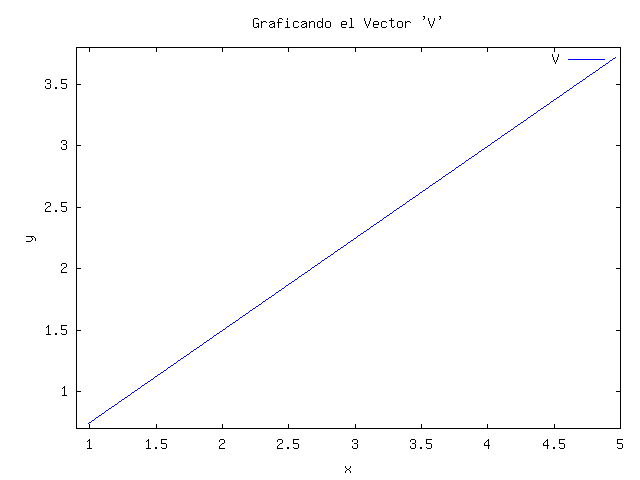
\includegraphics[scale=0.6]{imagenes/3_v.png}
	\newpage
	\item Al vector generado, aplique la transformación propuesta con argumento $17$, $31$, $47$,
		$61$, $97$, ¿Qué efecto puede ver?

		\textbf{R:}\\
	
		Analizando los gráficos:\\
		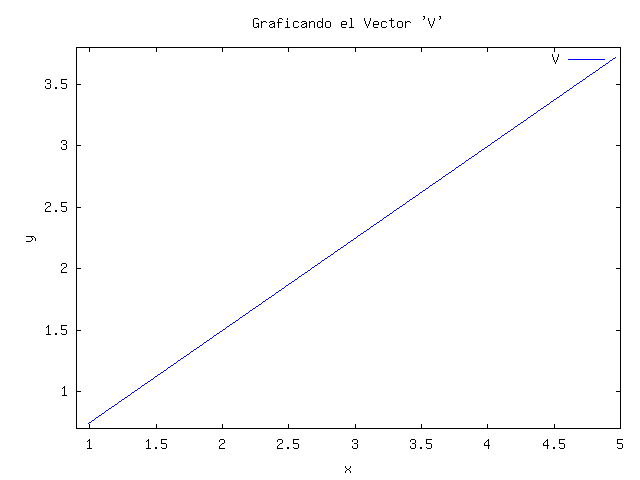
\includegraphics[scale=0.3]{imagenes/3_v.png}
		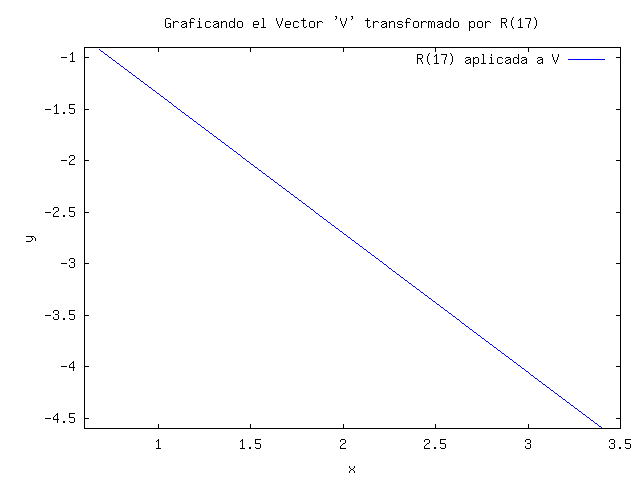
\includegraphics[scale=0.3]{imagenes/3_va.png}\\
		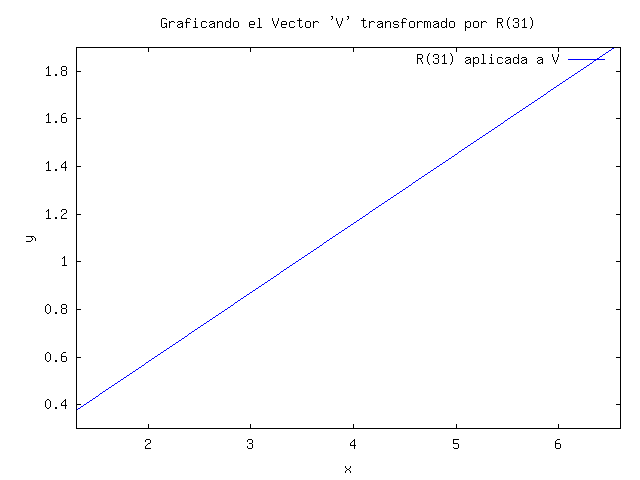
\includegraphics[scale=0.3]{imagenes/3_vb.png}
		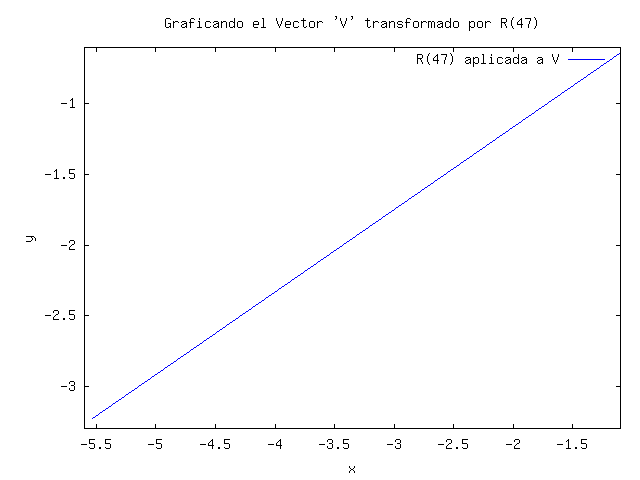
\includegraphics[scale=0.3]{imagenes/3_vc.png}\\
		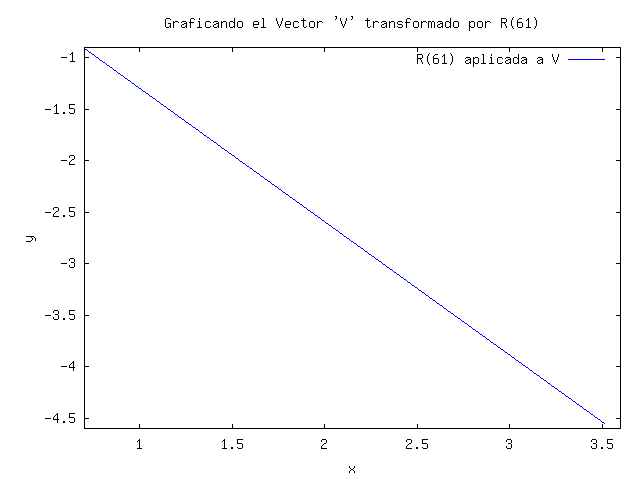
\includegraphics[scale=0.3]{imagenes/3_vd.png}
		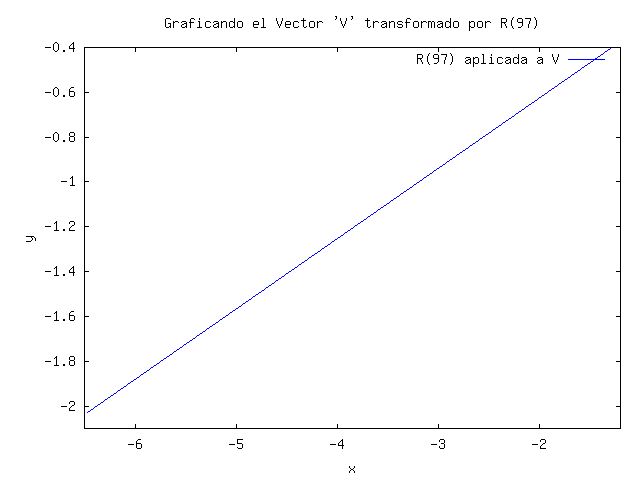
\includegraphics[scale=0.3]{imagenes/3_ve.png}
		
		Nos podemos dar cuenta que las transformaciones sólo rotan al vector sobre el eje de
		coordenadas.
		\newpage
	\item Realice el mismo ejercicio para un vector en $\Re^3$

		\textbf{R:}\\

		De la misma forma, generamos y graficamos un vector (ahora usando plot3):\\
		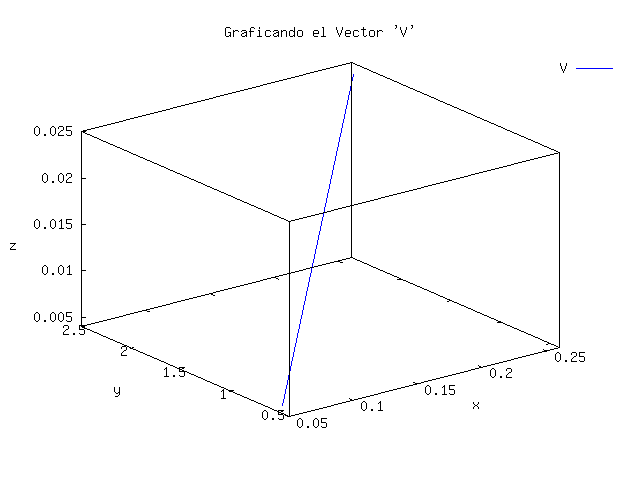
\includegraphics[scale=0.6]{imagenes/3_v3.png}

		Ahora, simplemente en vez de usar la matriz de transformación de $\Re^2$, la pasamos a
		$\Re^3$ dejando que al ser aplicada rote sobre el eje x:
		\[
		R_x(\theta) = \begin{bmatrix} 1 & 0 & 0 \\ 0 & \cos \theta	& -\sin \theta \\[3pt] 0 & \sin \theta  & \cos \theta \\[3pt] \end{bmatrix}\\[6pt] 
		\]

		\newpage
		Y revisando los gráficos:\\
		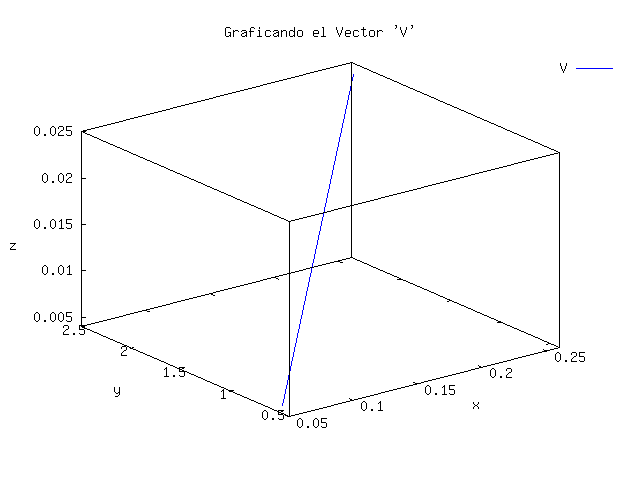
\includegraphics[scale=0.3]{imagenes/3_v3.png}
		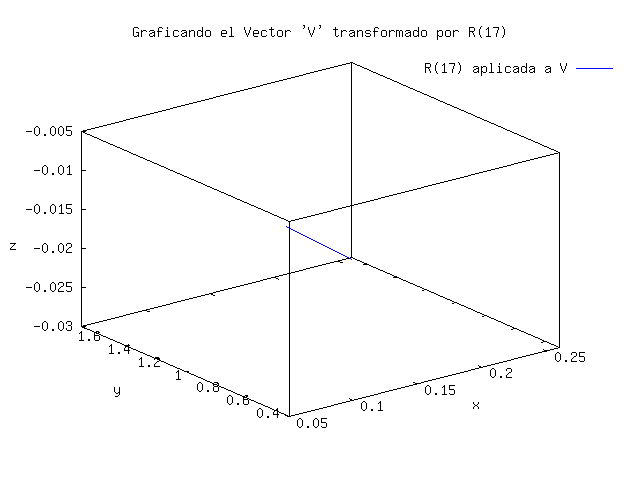
\includegraphics[scale=0.3]{imagenes/3_va3.png}\\
		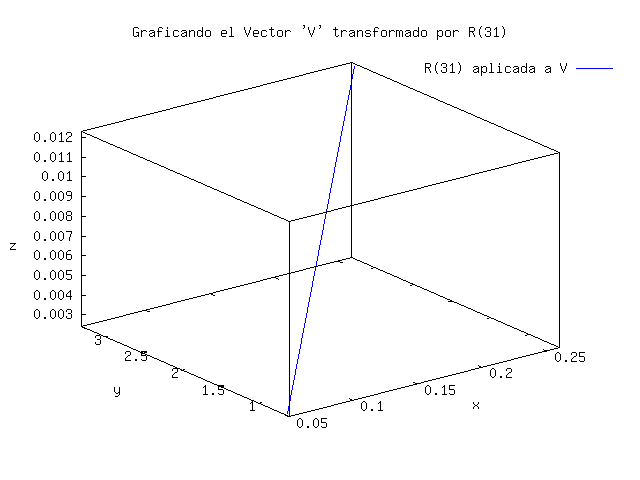
\includegraphics[scale=0.3]{imagenes/3_vb3.png}
		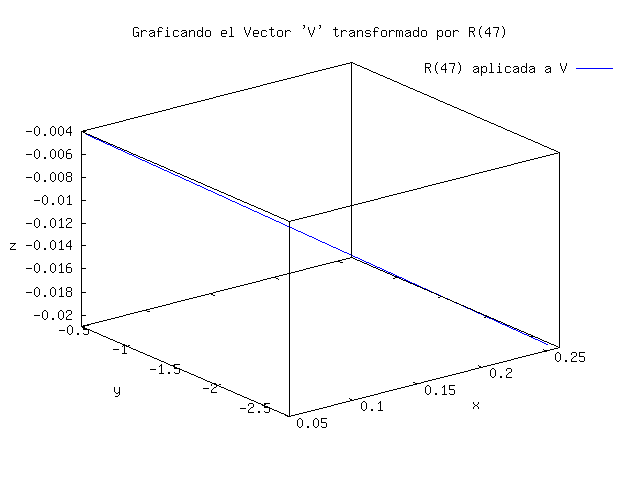
\includegraphics[scale=0.3]{imagenes/3_vc3.png}\\
		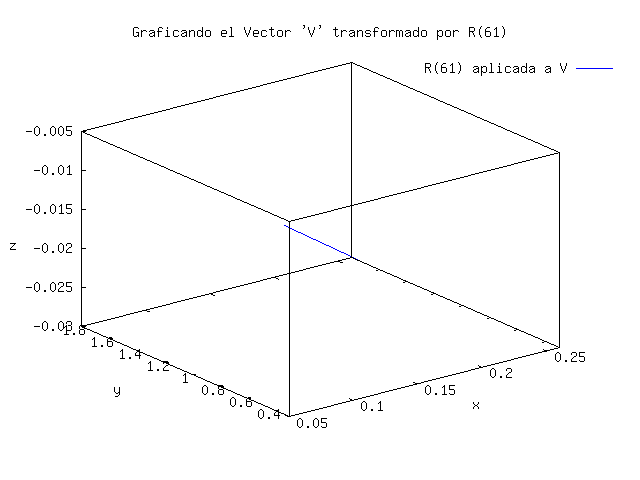
\includegraphics[scale=0.3]{imagenes/3_vd3.png}
		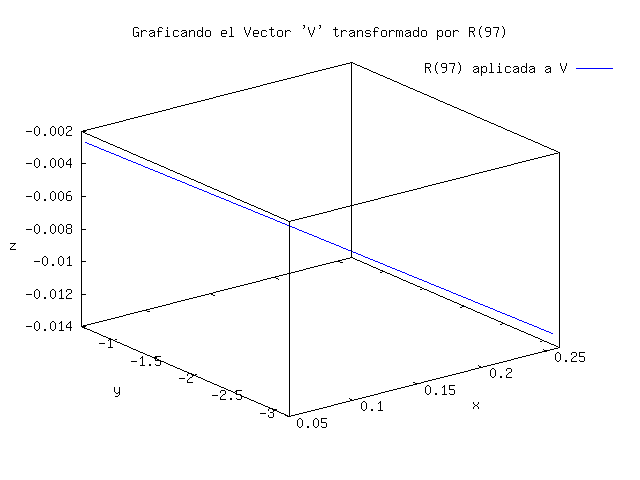
\includegraphics[scale=0.3]{imagenes/3_ve3.png}

		Podemos concluir que la transformación $R_x(\theta)$ en $\Re^3$, al igual que la transformación $R$
		en $\Re^2$, rota el vector en torno a los ejes de coordenadas.
\end{enumerate}

\newpage

\section{SVD}
\begin{enumerate}
	\item Implemente un algoritmo que calcule la factorización de svd.

	\textbf{R:}\\
	\begin{verbatim}

	function [U,S,V] = SVD(A)
		H = A'*A;
		[V,D] = eig(H);
		for i = 1:size(V)(1)
			D2(i,i) = sqrt(abs(D(i,i)));
		end
		for i = 1:size(D2)(1)
			j = size(D2)(1)+1-i;
			S(j,j) = D2(i,i);
		end
		for j = 1:size(V)(1)
			norma = 0;
			for i = 1:size(V)(1)
				norma = V(i,j)*V(i,j) + norma;
			end
			norma = sqrt(norma);
			for i = 1:size(V)(1)
				V(i,j) = V(i,j)/norma;
			end
		end
		s = size(V)(2);
		for j = 1:s
			for i = 1:s
				tmp(i,j) = V(i, s+1-j);
			end
		end
		V = tmp;
		U = A*V*inv(S);
	endfunction
	\end{verbatim}
	\newpage
	\item Compare su implementación con la que provee software como Octave. Para esto genere matrices
de tamaño superior a $101x101$ de forma aleatoria.

	\textbf{R:}\\

	Claramente la implementación que provee el software Octave, es mucho mas eficiente que el nuestro,
	especialmente en el tiempo que toma el calculo de la factorización. Además, notamos algunas
	diferencias (algunos cambios de signo), debido a la implementación de la función eig() que
	provee Octave, salvo en las matrices $\sum$, que contienen valores singulares idénticos.

\end{enumerate}


\newpage

\section{Conclusiones}
\subsection{Conclusiones Individuales}
%Conclusiones personales
Personalmente pude comprender la importancia de la sociedad en un individuo, sobre todo cuando Durkheim se refiere a que el suicidio es un hecho social y no un hecho individual,
la culpa no es del sujeto, es de la sociedad.

Otro aspecto importante es como la sociedad nos ense\~na a actuar, a pensar, todo respecto a sus mismos est\'andares, y la sociedad castiga muy duramente a quien no act\'ua como
ella misma le ense\~no, un aspecto muy claro que se puede apreciar mirando una cultura determinada, el extremismo y como muchas personas viven con sus ojos vendados, aceptando
una verdad local, que a los ojos del resto del mundo puede estar erroneo, pero ?`No es el resto del mundo otra macro-cultura que también nos obliga a pensar de una forma?

Principalmente, pude darme cuenta que la visi\'on que ten\'ia Durkheim con respecto a la sociedad, fue una marca intachable en la historia del pensamiento humano,
ya que el separandose de todos los aspectos posibles, dejando atr\'as emociones, prejuicios, creencias, pudo generar un juicio imparcial para poder formar o declarar
la sociolog\'ia actual como una ciencia, que hoy en d\'ia es una de las ciencias mas importantes para el estudio de la humanidad

Finalmente, a nivel  personal me llamo mucho la atenci\'on como pudo tener la valent\'ia en su tiempo de poder analizar fen\'omenos sociales, sin ninguna influencia tan notoria
dejando de lado pensamiento que ven\'ian de 8 generaciones antes que el a nivel familiar, y que si nos damos cuenta claramente son la estructura de la organizaci\'on llamada sociedad.
Sin dejar de lado, la capacidad que tuvo para poder describir que una organizaci\'on se puede llevar a la autodestrucci\'on (Anomia), t\'ermino que sirvi\'o y sirve notablemente al
momento de analizar los riesgos de las organizaciones actuales.



\subsection{Conclusiones Generales}
%Conclusiones 'en conjunto' ......

La visi\'on de Durkheim de la sociedad marc\'o al pensamiento mundial en una manera que era
muy necesaria, dejar de lado todo tipo de prejuicios y emociones para generar un juicio imparcial y
racional de \'esta se volvio el pilar de la Sociolog\'ia, ciencia que hoy en dia se ha establecido como
una de las mas importantes de las Ciencias Sociales.

A trav\'es de las ideas del autor, las empresas se pueden analizar con ``sangre fr\'ia'', extrapolan-
do las ideas de ``hechos sociales'' y ``estructura'' a organizaciones mas pequeñas. De esta manera se
puede entender mejor la forma de comportarse de algunas organizaciones que tienden
a la autodestrucci\'on o que logran surgir en ambientes altamente hostiles.

%	\item Sobre los hechos sociales
Adem\'as, cuando uno es insertado en una nueva comunidad, como lo es una organizaci\'on o empresa hoy en d\'ia, uno 
se ve rodeado de un sistema con una cultura propia y muchas veces diferente a la del individuo. Estos 
detalles impl\'icitos muchas veces dentro dela organizaci\'on, son los reconocidos como ``hechos sociales''
por Durkheim. Por ello, podemos concluir que fue importante que Durkheim halla reconocido que los 
hechos sociales deb\'ian ser analisados por m\'etodos diferentes a los de la psicolog\'ia, ya que los estudios 
de sociolog\'ia desarrollados por \'el han sido un gran aporte para el estudio de la administraci\'on general 
de estos ``sistemas humanos'', jugando un rol medular en el asunto. 

%	\item Sobre las Corrientes Sociales\\
Tambi\'en, esto dicho anteriormente  deber\'iamos encararlo con objetividad, desprendiéndonos de todos los prejuicios y preconceptos que podamos tener antes de abordarlos.\\
Esto puede llegar a ser muy difícil, si a modo de ejemplo tomamos por punto de partida que el analista pertenece a una colectividad, a una sociedad, que tiene determinado su pensamiento a través del lenguaje que determina en sí mismo una estructura preestablecida de pensamiento lógico.


%	\item Sobre la divisi\'on del trabajo social\\
Para el estudio y administraci\'on de empresas u organizaciones, el concepto de solidaridad desarrollado
por Durkheim es importante de recalcar. Vi\'endolo desde su punto de vista, cada organizaci\'on deber\'ia 
buscar una solidaridad mec\'anica entre sus miembros. De esta forma, los individuos lograr\'ian adquirir 
una mentalidad enfocada a los objetivos de la empresa (vista como comunidad), y as\'i, mantener un 
ambiente de unidad y confianza en torno a los ideales de \'esta. Es notable mencionar que muchas 
organizaciones tienden a de hoy en dia tienden a fomentar un ambiente competitivo entre sus integrantes, 
lo cual, al igual que la mentalidad individualista en la realidad actual, conlleva muchas veces a problemas 
t\'ipicos de una solidaridad org\'anica.

%	\item  Sobre la educaci\'on\\
Ahora si analizamos las las funciones de la educaci\'on destacadas por Durkheim, desde el punto de vista de las organizaciones, 
la educaci\'on sirve como herramienta para lograr un mayor orden social, una mayor lealtad y una mayor especializaci\'on 
de los integrantes hacia la comunidad, siendo as\'i de gran importancia para mejorar la integraci\'on de nuevos miembros
y el crecimiento de la empresa.
	
%	\item  Sobre el Crimen
%Durkheim identific\'o al crimen como un indicador de la necesidad de cambios dentro de las organizaciones. 

%	\item Sobre la Ley
%Postulados principales:
% Diferencia duramente entre el Individualismo y la avaricia y el egoismo
% Avaricia y egoismo no son en lo absoluto posturas morales
% Estudia la Ley como una expresi\'on que garantizaba los valores fundamentales de la sociedad.

%	\item Sobre el Suicidio\\
De la misma manera, Durkheim, con su trabajo sobre el suicidio de los individuos con diferentes hechos sociales, logra destacar como ciertos 
factores en la sociedad (debilitamiento de los lazos de integraci\'on, desregularizaci\'on moral y falta de definiciones 
leg\'itimas, sociedades muy opresivas) pueden llevar a la autodestrucci\'on de sus miembros.\\
Por ello, se puede concluir que  es importante que las organizaciones se preocupen de mantener a sus integrantes 
cuidando de no desarrollar estas fallas que requieren de una reconstrucci\'on social.

%	\item Sobre la Religi\'on\\
Por \'ultimo, sus estudios sobre la religi\'on permitieron comprender mejor el desarrollo del orden social en las primeras comunidades, 
cumpliendo estas la funci\'on de separar lo mundano o cotidiano de las cosas intangibles, que relacionadas con lo sagrado, 
lograban la generaci\'on de normas que fomentaban el orden social.



\newpage

\newpage


\end{document}
